\documentclass[11pt]{amsbook}

\usepackage[turkish]{babel}
\usepackage{../Ceyhun}
\usepackage{../amsTurkish}

\begin{document}
\hPage{122}

Örneğin, Şekil \ref{fig:1}
deki çizgeyi düşünelim. ($a_1$, $a_2$, $a_3$) kümesi de çizgeyi iki parçaya parçalayacağından bu çizgedeki ($a_1$, $a_2$, $a_3$, $a_6$) kümesi bir kesitleme değildir. Çizgeyi üç parçaya parçalayacağından, ($a_3$, $a_4$, $a_7$) kümesi de bir kesitleme değildir. Beri yanda,

\[
	K_1 = (a_3, a_4)
\]
\[
	K_2 = (a_7)
\]
\[
	K_3 = (a_1, a_2, a_4)
\]

kümeleri birer kesitlemedir.

\[
	K_4 = K_1 \oplus K_3
\]
\[
	      = (a_1, a_2, a_3)	
\]

kümesi de bir kesitlemedir.

\[
	K_5 = K_1 \oplus K_2
\]
\[
	      = (a_3, a_4, a_7)	
\]

ise ortak ayrıtsız iki kesitlemeden oluşan bir kümedir.

\begin{figure}[htbp]
\begin{center}
	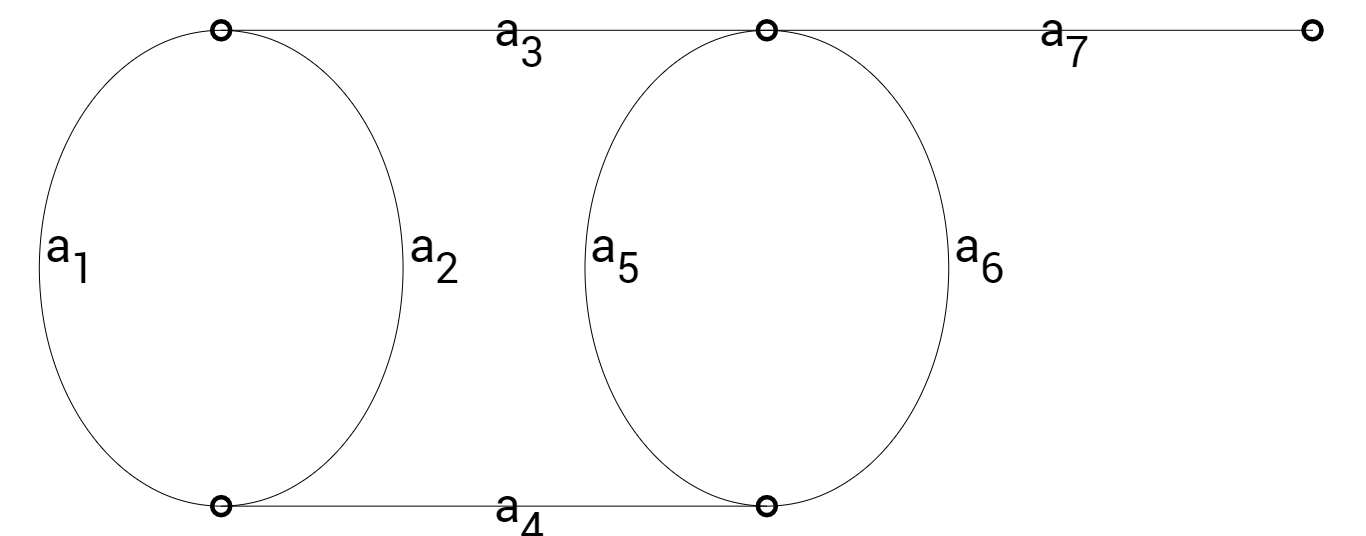
\includegraphics [ width=0.5\columnwidth ]{images/ceyhun-122-fig01.png}
	\caption{Kesitleme kavramının açıklanması.}
	\label{fig:1}
\end{center}
\end{figure}
 

\end{document}